% answers.tex —— 2005 年·普通高等学校招生考试·福建卷·理科 · 参考答案与详细解析片段
% 由 tools/generate_projects.py 依来源总账自 2005/2005_数学真题_福建理科_试题.md + 2005/2005_数学真题_福建理科_解析正文.md + 2005/2005_数学真题_福建理科_答案要点.md 生成，勿手改（改源 MD 后重跑）

\gkpart{一、选择题}

\begin{answer}
\gksolhead{1}{}

\textbf{题目}：

复数 $z = \dfrac{1}{1-\mathrm{i}}$ 的共轭复数是\mbox{（　　）}

\begin{gkopts}(2)
\task A．$\dfrac{1}{2} + \dfrac{1}{2}\mathrm{i}$
\task B．$\dfrac{1}{2} - \dfrac{1}{2}\mathrm{i}$
\task C．$1 - \mathrm{i}$
\task D．$1 + \mathrm{i}$
\end{gkopts}

\Needspace{4\baselineskip}
\textbf{解析}

\Needspace{5\baselineskip}
计算复数 $z$ 的代数形式：
\nopagebreak[4]
\[
z = \frac{1}{1-\mathrm{i}} = \frac{1+\mathrm{i}}{(1-\mathrm{i})(1+\mathrm{i})} = \frac{1+\mathrm{i}}{1 - \mathrm{i}^2} = \frac{1+\mathrm{i}}{2} = \frac{1}{2} + \frac{1}{2}\mathrm{i}.
\]
\Needspace{5\baselineskip}
根据共轭复数的定义，虚部变号，得其共轭复数：
\nopagebreak[4]
\[
\bar{z} = \frac{1}{2} - \frac{1}{2}\mathrm{i}.
\]
故选 B．

\gkanswer{答案：B}

\end{answer}
\begin{answer}
\gksolhead{2}{}

\textbf{题目}：

已知等差数列 $\{a_n\}$ 中，$a_7 + a_9 = 16$，$a_4 = 1$，则 $a_{12}$ 的值是\mbox{（　　）}

\begin{gkopts}(4)
\task A．$15$
\task B．$30$
\task C．$31$
\task D．$64$
\end{gkopts}

\Needspace{4\baselineskip}
\textbf{解析}

设等差数列 $\{a_n\}$ 的公差为 $d$．
\Needspace{5\baselineskip}
由等差数列的性质，下标和相等性质：
\nopagebreak[4]
\[
a_7 + a_9 = 2a_8 = 16 \implies a_8 = 8.
\]
\Needspace{5\baselineskip}
已知 $a_4 = 1$，则：
\nopagebreak[4]
\[
a_8 - a_4 = 4d = 8 - 1 = 7.
\]
\Needspace{5\baselineskip}
因此：
\nopagebreak[4]
\[
a_{12} = a_8 + 4d = 8 + 7 = 15.
\]
故选 A．

\gkanswer{答案：A}

\end{answer}
\begin{answer}
\gksolhead{3}{}

\textbf{题目}：

在 $\triangle ABC$ 中，$\angle C = 90^\circ$，$\overrightarrow{AB} = (k, 1)$，$\overrightarrow{AC} = (2, 3)$，则 $k$ 的值是\mbox{（　　）}

\begin{gkopts}(4)
\task A．$5$
\task B．$-5$
\task C．$\dfrac{3}{2}$
\task D．$-\dfrac{3}{2}$
\end{gkopts}

\Needspace{4\baselineskip}
\textbf{解析}

在 $\triangle ABC$ 中，已知 $\overrightarrow{AB} = (k, 1)$，$\overrightarrow{AC} = (2, 3)$．
\Needspace{5\baselineskip}
由向量减法的三角形法则：
\nopagebreak[4]
\[
\overrightarrow{CB} = \overrightarrow{AB} - \overrightarrow{AC} = (k - 2, 1 - 3) = (k - 2, -2).
\]
又 $\overrightarrow{CA} = -\overrightarrow{AC} = (-2, -3)$．
\Needspace{5\baselineskip}
因为 $\angle C = 90^\circ$，所以 $\overrightarrow{CA} \perp \overrightarrow{CB}$，其数量积为零：
\nopagebreak[4]
\[
\overrightarrow{CA} \cdot \overrightarrow{CB} = (-2)(k - 2) + (-3)(-2) = -2k + 4 + 6 = 10 - 2k = 0.
\]
解得 $k = 5$．
故选 A．

\gkanswer{答案：A}

\end{answer}
\begin{answer}
\gksolhead{4}{}

\textbf{题目}：

已知直线 $m$、$n$ 与平面 $\alpha, \beta$，给出下列三个命题：
① 若 $m \parallel \alpha, n \parallel \alpha$，则 $m \parallel n$；
② 若 $m \parallel \alpha, n \perp \alpha$，则 $n \perp m$；
③ 若 $m \perp \alpha, m \parallel \beta$，则 $\alpha \perp \beta$．
其中真命题的个数是\mbox{（　　）}

\begin{gkopts}(4)
\task A．$0$
\task B．$1$
\task C．$2$
\task D．$3$
\end{gkopts}

\Needspace{4\baselineskip}
\textbf{解析}

逐项分析各命题：
\begin{itemize}
\item 对于 ①：若 $m \parallel \alpha$，$n \parallel \alpha$，在空间中平行于同一平面的两条直线可以平行、相交或异面，故 ① 为假命题；
\item 对于 ②：若 $m \parallel \alpha$，$n \perp \alpha$，由线面平行的性质，平面 $\alpha$ 内必存在直线 $l$ 使得 $l \parallel m$．因为 $n \perp \alpha$，所以 $n \perp l$，进而由平行性质得 $n \perp m$，故 ② 为真命题；
\item 对于 ③：若 $m \perp \alpha$，$m \parallel \beta$，过直线 $m$ 作平面与 $\beta$ 相交于直线 $b$，则 $b \parallel m$．因为 $m \perp \alpha$，所以 $b \perp \alpha$．又因为 $b \subset \beta$，由面面垂直判定定理可得 $\alpha \perp \beta$，故 ③ 为真命题．
\end{itemize}

真命题的个数为 2．
故选 C．

\gkanswer{答案：C}

\end{answer}
\begin{answer}
\gksolhead{5}{}

\textbf{题目}：

若函数 $f(x) = a^{x-b}$ 的图象如图，其中 $a, b$ 为常数，则下列结论正确的是\mbox{（　　）}
\nopagebreak[4]
\begin{center}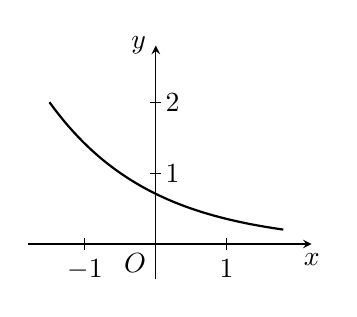
\begin{tikzpicture}[>=stealth, scale=0.9]
  % 坐标轴
  \draw[->] (-1.8, 0) -- (2.2, 0) node[below] {$x$};
  \draw[->] (0, -0.5) -- (0, 2.8) node[left] {$y$};
  \node[below left] at (0, 0) {$O$};

  % 刻度
  \draw (-1, 0.08) -- (-1, -0.08) node[below] {$-1$};
  \draw (1, 0.08) -- (1, -0.08) node[below] {$1$};
  \draw (0.08, 1) -- (-0.08, 1);
  \node[right] at (0, 1) {$1$};
  \draw (0.08, 2) -- (-0.08, 2);
  \node[right] at (0, 2) {$2$};

  % 指数函数曲线 (a=0.5, b=-0.5 即 y = 0.5^(x + 0.5))
  \draw[thick, domain=-1.5:1.8, samples=50] plot (\x, {pow(0.5, \x + 0.5)});
\end{tikzpicture}
\end{center}
\nopagebreak[4]
\begin{gkopts}(2)
\task A．$a > 1, b < 0$
\task B．$a > 1, b > 0$
\task C．$0 < a < 1, b > 0$
\task D．$0 < a < 1, b < 0$
\end{gkopts}

\Needspace{4\baselineskip}
\textbf{解析}

观察函数 $f(x) = a^{x-b}$ 的图象：
1. 函数图象在 $\mathbf{R}$ 上严格单调递减，根据指数函数的性质，底数满足 $0 < a < 1$；
\Needspace{5\baselineskip}
2. 当 $x = 0$ 时，$f(0) = a^{-b}$．从图象可见，$y$ 轴上的截距严格介于 $0$ 与 $1$ 之间，即：
\nopagebreak[4]
\[
0 < a^{-b} < 1 = a^0.
\]
\Needspace{5\baselineskip}
因为底数 $0 < a < 1$，由指数不等式的单调性可得：
\nopagebreak[4]
\[
-b > 0 \implies b < 0.
\]
（亦可由特征点分析：令 $a^{x-b} = 1$ 得 $x = b$，图象上函数值为 1 的点横坐标位于负半轴，故 $b < 0$）．
综上所述，$0 < a < 1, b < 0$．
故选 D．

\gkanswer{答案：D}

\end{answer}
\begin{answer}
\gksolhead{6}{}

\textbf{题目}：

若函数 $y = \sin(\omega x + \varphi) \; (x \in \mathbf{R}, \omega > 0, 0 \leqslant \varphi < 2\pi)$ 的部分图象如图，则\mbox{（　　）}
\nopagebreak[4]
\begin{center}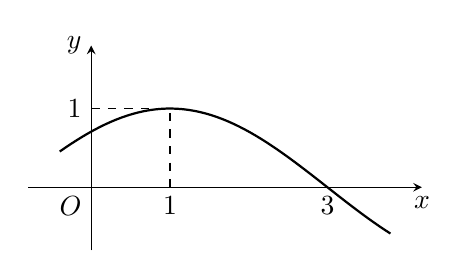
\begin{tikzpicture}[>=stealth, scale=1.0]
  % 坐标轴
  \draw[->] (-0.8, 0) -- (4.2, 0) node[below] {$x$};
  \draw[->] (0, -0.8) -- (0, 1.8) node[left] {$y$};
  \node[below left] at (0, 0) {$O$};

  % 刻度与虚线
  \node[left] at (0, 1) {$1$};
  \node[below] at (1, 0) {$1$};
  \node[below] at (3, 0) {$3$};

  \draw[dashed] (0, 1) -- (1, 1) -- (1, 0);

  % 正弦函数曲线: y = sin(pi/4 * x + pi/4)
  \draw[thick, domain=-0.4:3.8, samples=60] plot (\x, {sin((\x * 0.25 + 0.25) * 180)});
\end{tikzpicture}
\end{center}
\nopagebreak[4]
\begin{gkopts}(1)
\task A．$\omega = \dfrac{\pi}{2}, \varphi = \dfrac{\pi}{4}$
\task B．$\omega = \dfrac{\pi}{3}, \varphi = \dfrac{\pi}{6}$
\task C．$\omega = \dfrac{\pi}{4}, \varphi = \dfrac{\pi}{4}$
\task D．$\omega = \dfrac{\pi}{4}, \varphi = \dfrac{5\pi}{4}$
\end{gkopts}

\Needspace{4\baselineskip}
\textbf{解析}

由函数 $y = \sin(\omega x + \varphi) \; (\omega > 0, 0 \leqslant \varphi < 2\pi)$ 的部分图象可知：
波峰位于点 $(1, 1)$，与其相邻的右侧零点位于点 $(3, 0)$．
\Needspace{5\baselineskip}
两点横坐标之差等于四分之一周期：
\nopagebreak[4]
\[
\frac{T}{4} = 3 - 1 = 2 \implies T = 8.
\]
\Needspace{5\baselineskip}
由周期公式：
\nopagebreak[4]
\[
\omega = \frac{2\pi}{T} = \frac{2\pi}{8} = \frac{\pi}{4}.
\]
\Needspace{5\baselineskip}
因为点 $(1, 1)$ 为图象的最高点，代入解析式：
\nopagebreak[4]
\[
\sin\left(\frac{\pi}{4} \times 1 + \varphi\right) = 1.
\]
\Needspace{5\baselineskip}
因此：
\nopagebreak[4]
\[
\frac{\pi}{4} + \varphi = \frac{\pi}{2} + 2k\pi \quad (k \in \mathbf{Z}) \implies \varphi = \frac{\pi}{4} + 2k\pi.
\]
结合题设条件 $0 \leqslant \varphi < 2\pi$，取 $k = 0$，得 $\varphi = \dfrac{\pi}{4}$．
故选 C．

\gkanswer{答案：C}

\end{answer}
\begin{answer}
\gksolhead{7}{}

\textbf{题目}：

已知 $p: |2x - 3| < 1$，$q: x(x - 3) < 0$，则 $p$ 是 $q$ 的\mbox{（　　）}

\begin{gkopts}(2)
\task A．充分不必要条件
\task B．必要不充分条件
\task C．充要条件
\task D．既不充分也不必要条件
\end{gkopts}

\Needspace{4\baselineskip}
\textbf{解析}

分别解两个条件：
\begin{itemize}
\item 由 $p: |2x - 3| < 1$ 得：
\end{itemize}
\nopagebreak[4]
\[
-1 < 2x - 3 < 1 \iff 2 < 2x < 4 \iff 1 < x < 2.
\]
其解集为区间 $A = (1, 2)$．
\begin{itemize}
\item 由 $q: x(x - 3) < 0$ 得：
\end{itemize}
\nopagebreak[4]
\[
0 < x < 3.
\]
其解集为区间 $B = (0, 3)$．

显然 $A \subsetneqq B$，即 $(1, 2) \subsetneqq (0, 3)$．
因此 $p \implies q$，但 $q \nRightarrow p$．
所以 $p$ 是 $q$ 的充分不必要条件．
故选 A．

\gkanswer{答案：A}

\end{answer}
\begin{answer}
\gksolhead{8}{}

\textbf{题目}：

如图，长方体 $ABCD - A_1B_1C_1D_1$ 中，$AA_1 = AB = 2$，$AD = 1$，点 $E$、$F$、$G$ 分别是 $DD_1$、$AB$、$CC_1$ 的中点，则异面直线 $A_1E$ 与 $GF$ 所成的角是\mbox{（　　）}
\nopagebreak[4]
\begin{center}\begin{tikzpicture}[>=stealth, scale=1.0]
  % 顶点定义
  \coordinate (A) at (0, 0);
  \coordinate (B) at (2.4, 0);
  \coordinate (C) at (3.4, 0.8);
  \coordinate (D) at (1.0, 0.8);
  \coordinate (A1) at (0, 2.2);
  \coordinate (B1) at (2.4, 2.2);
  \coordinate (C1) at (3.4, 3.0);
  \coordinate (D1) at (1.0, 3.0);

  % 中点定义
  \coordinate (E) at ($(D)!0.5!(D1)$);
  \coordinate (F) at ($(A)!0.5!(B)$);
  \coordinate (G) at ($(C)!0.5!(C1)$);

  % 可见实线
  \draw[thick] (A) -- (B) -- (C) -- (C1) -- (D1) -- (A1) -- cycle;
  \draw[thick] (B) -- (B1) -- (C1);
  \draw[thick] (A1) -- (B1);

  % 不可见虚线
  \draw[thick, dashed] (A) -- (D) -- (C);
  \draw[thick, dashed] (D) -- (D1);

  % 异面直线连接
  \draw[thick, dashed] (A1) -- (E);
  \draw[thick, dashed] (G) -- (F);

  % 顶点标签
  \node[below left] at (A) {$A$};
  \node[below right] at (B) {$B$};
  \node[right] at (C) {$C$};
  \node[above left] at (D) {$D$};
  \node[above left] at (A1) {$A_1$};
  \node[below left] at (B1) {$B_1$};
  \node[above right] at (C1) {$C_1$};
  \node[above left] at (D1) {$D_1$};
  \node[right] at (E) {$E$};
  \node[below] at (F) {$F$};
  \node[right] at (G) {$G$};
\end{tikzpicture}
\end{center}
\nopagebreak[4]
\begin{gkopts}(2)
\task A．$\arccos\dfrac{\sqrt{15}}{5}$
\task B．$\dfrac{\pi}{4}$
\task C．$\arccos\dfrac{\sqrt{10}}{5}$
\task D．$\dfrac{\pi}{2}$
\end{gkopts}

\Needspace{4\baselineskip}
\textbf{解析}

以点 $D$ 为坐标原点，分别以 $\overrightarrow{DA}$、$\overrightarrow{DC}$、$\overrightarrow{DD_1}$ 的方向为 $x$ 轴、$y$ 轴、$z$ 轴的正方向建立空间直角坐标系．
已知 $AA_1 = AB = 2$，$AD = 1$．
各顶点坐标为：
$D(0, 0, 0)$，$A(1, 0, 0)$，$B(1, 2, 0)$，$C(0, 2, 0)$，
$A_1(1, 0, 2)$，$B_1(1, 2, 2)$，$C_1(0, 2, 2)$，$D_1(0, 0, 2)$．
点 $E$、$F$、$G$ 分别是 $DD_1$、$AB$、$CC_1$ 的中点，由中点坐标公式：
$E(0, 0, 1)$，$F(1, 1, 0)$，$G(0, 2, 1)$．
\Needspace{5\baselineskip}
计算向量：
\nopagebreak[4]
\[
\overrightarrow{A_1E} = (0 - 1, 0 - 0, 1 - 2) = (-1, 0, -1),
\]
\nopagebreak[4]
\[
\overrightarrow{GF} = (1 - 0, 1 - 2, 0 - 1) = (1, -1, -1).
\]
\Needspace{5\baselineskip}
计算两向量的数量积：
\nopagebreak[4]
\[
\overrightarrow{A_1E} \cdot \overrightarrow{GF} = (-1) \times 1 + 0 \times (-1) + (-1) \times (-1) = -1 + 0 + 1 = 0.
\]
因为数量积为 0，所以两直线垂直，异面直线 $A_1E$ 与 $GF$ 所成的角是 $\dfrac{\pi}{2}$．
故选 D．

\gkanswer{答案：D}

\end{answer}
\begin{answer}
\gksolhead{9}{}

\textbf{题目}：

从 6 人中选 4 人分别到巴黎、伦敦、悉尼、莫斯科四个城市游览，要求每个城市有一人游览，每人只游览一个城市，且这 6 人中甲、乙两人不去巴黎游览，则不同的选择方案共有\mbox{（　　）}

\begin{gkopts}(4)
\task A．$300$ 种
\task B．$240$ 种
\task C．$144$ 种
\task D．$96$ 种
\end{gkopts}

\Needspace{4\baselineskip}
\textbf{解析}

分两步安排：
第一步：从除甲、乙之外的其余 4 人中选 1 人去巴黎游览，有 $\mathrm{C}_4^1 = 4$ 种选法；
第二步：从剩下的 5 人中选 3 人分别去伦敦、悉尼、莫斯科游览，这是一排列问题，共有 $\mathrm{A}_5^3 = 5 \times 4 \times 3 = 60$ 种方案．
\Needspace{5\baselineskip}
根据分步乘法计数原理，不同的选择方案总数为：
\nopagebreak[4]
\[
N = 4 \times 60 = 240 \text{ \text{种}}.
\]
故选 B．

\gkanswer{答案：B}

\end{answer}
\begin{answer}
\gksolhead{10}{}

\textbf{题目}：

已知 $F_1$、$F_2$ 是双曲线 $\dfrac{x^2}{a^2} - \dfrac{y^2}{b^2} = 1 \; (a > 0, b > 0)$ 的两焦点，以线段 $F_1F_2$ 为边作正三角形 $MF_1F_2$，若边 $MF_1$ 的中点在双曲线上，则双曲线的离心率是\mbox{（　　）}

\begin{gkopts}(2)
\task A．$4 + 2\sqrt{3}$
\task B．$\sqrt{3} - 1$
\task C．$\dfrac{\sqrt{3} + 1}{2}$
\task D．$\sqrt{3} + 1$
\end{gkopts}

\Needspace{4\baselineskip}
\textbf{解析}

双曲线两焦点为 $F_1(-c, 0)$、$F_2(c, 0)$，焦距 $|F_1F_2| = 2c$．
$\triangle MF_1F_2$ 是以线段 $F_1F_2$ 为底边的正三角形，其边长为 $2c$．
点 $P$ 为边 $MF_1$ 的中点，所以在正三角形中，$F_1P = \dfrac{1}{2}MF_1 = c$．
且由正三角形中线即高的性质，$F_2P \perp MF_1$．
在 Rt$\triangle F_1PF_2$ 中，斜边 $|F_1F_2| = 2c$，直角边 $|PF_1| = c$，
\Needspace{5\baselineskip}
由勾股定理可得另一条直角边：
\nopagebreak[4]
\[
|PF_2| = \sqrt{(2c)^2 - c^2} = \sqrt{3}c.
\]
\Needspace{5\baselineskip}
点 $P$ 在双曲线上，根据双曲线的定义，两焦点到双曲线上点 $P$ 的距离之差的绝对值等于 $2a$：
\nopagebreak[4]
\[
|PF_2| - |PF_1| = \sqrt{3}c - c = (\sqrt{3} - 1)c = 2a.
\]
\Needspace{5\baselineskip}
因此双曲线的离心率为：
\nopagebreak[4]
\[
e = \frac{c}{a} = \frac{2}{\sqrt{3} - 1} = \frac{2(\sqrt{3} + 1)}{(\sqrt{3} - 1)(\sqrt{3} + 1)} = \sqrt{3} + 1.
\]
故选 D．

\gkanswer{答案：D}

\end{answer}
\begin{answer}
\gksolhead{11}{}

\textbf{题目}：

设 $a, b \in \mathbf{R}$，$a^2 + 2b^2 = 6$，则 $a + b$ 的最小值是\mbox{（　　）}

\begin{gkopts}(2)
\task A．$-2\sqrt{2}$
\task B．$-\dfrac{5\sqrt{3}}{3}$
\task C．$-3$
\task D．$-\dfrac{7}{2}$
\end{gkopts}

\Needspace{4\baselineskip}
\textbf{解析}

\Needspace{5\baselineskip}
由柯西不等式：
\nopagebreak[4]
\[
(a + b)^2 = \left(1 \cdot a + \frac{1}{\sqrt{2}} \cdot (\sqrt{2}b)\right)^2 \leqslant \left(1^2 + \left(\frac{1}{\sqrt{2}}\right)^2\right) (a^2 + 2b^2).
\]
\Needspace{5\baselineskip}
代入 $a^2 + 2b^2 = 6$：
\nopagebreak[4]
\[
(a + b)^2 \leqslant \left(1 + \frac{1}{2}\right) \times 6 = \frac{3}{2} \times 6 = 9.
\]
\Needspace{5\baselineskip}
因此：
\nopagebreak[4]
\[
-3 \leqslant a + b \leqslant 3.
\]
当且仅当 $\dfrac{a}{1} = \dfrac{\sqrt{2}b}{1/\sqrt{2}}$，即 $a = 2b$ 时等号成立．
将 $a = 2b$ 代入 $a^2 + 2b^2 = 6$，得 $4b^2 + 2b^2 = 6 \implies b^2 = 1$．
取 $b = -1$，$a = -2$ 时，$a + b = -3$ 取得最小值．
故选 C．

\gkanswer{答案：C}

\end{answer}
\begin{answer}
\gksolhead{12}{}

\textbf{题目}：

$f(x)$ 是定义在 $\mathbf{R}$ 上的以 3 为周期的奇函数，且 $f(2) = 0$，则方程 $f(x) = 0$ 在区间 $(0, 6)$ 内解的个数的最小值是\mbox{（　　）}

\begin{gkopts}(4)
\task A．$2$
\task B．$3$
\task C．$5$
\task D．$7$
\end{gkopts}

\Needspace{4\baselineskip}
\textbf{解析}

已知 $f(x)$ 是定义在 $\mathbf{R}$ 上的奇函数，所以 $f(0) = 0$．
\Needspace{5\baselineskip}
又 $f(x)$ 的周期为 3，所以：
\nopagebreak[4]
\[
f(3) = f(0) = 0, \quad f(6) = f(3) = 0.
\]
\Needspace{5\baselineskip}
已知 $f(2) = 0$，由周期为 3 可得：
\nopagebreak[4]
\[
f(-1) = f(2 - 3) = f(2) = 0, \quad f(5) = f(2 + 3) = f(2) = 0.
\]
\Needspace{5\baselineskip}
又因为 $f(x)$ 是奇函数，所以：
\nopagebreak[4]
\[
f(1) = -f(-1) = 0.
\]
\Needspace{5\baselineskip}
再由周期为 3 可得：
\nopagebreak[4]
\[
f(4) = f(1 + 3) = f(1) = 0.
\]
因此，在开区间 $(0, 6)$ 内，函数 $f(x)$ 至少有 $x = 1, 2, 3, 4, 5$ 共 5 个互不相同的零点．
故方程 $f(x) = 0$ 在区间 $(0, 6)$ 内解的个数的最小值是 5．
故选 C．

\gkanswer{答案：C}

\end{answer}
\gkpart{二、填空题}

\begin{answer}
\gksolhead{13}{}

\textbf{题目}：

$\left(2\sqrt{x} - \dfrac{1}{x}\right)^6$ 展开式中的常数项是 $\underline{\qquad\qquad}$．（用数字作答）

\Needspace{4\baselineskip}
\textbf{解析}

\Needspace{5\baselineskip}
二项式 $\left(2\sqrt{x} - \dfrac{1}{x}\right)^6$ 展开式的通项公式为：
\nopagebreak[4]
\[
T_{r+1} = \mathrm{C}_6^r (2\sqrt{x})^{6-r} \left(-\frac{1}{x}\right)^r = \mathrm{C}_6^r 2^{6-r} (-1)^r x^{\frac{6-r}{2} - r} = \mathrm{C}_6^r 2^{6-r} (-1)^r x^{3 - \frac{3}{2}r}.
\]
\Needspace{5\baselineskip}
令 $x$ 的指数为 0：
\nopagebreak[4]
\[
3 - \frac{3}{2}r = 0 \implies r = 2.
\]
\Needspace{5\baselineskip}
代入计算常数项：
\nopagebreak[4]
\[
T_3 = \mathrm{C}_6^2 2^{6-2} (-1)^2 = 15 \times 16 \times 1 = 240.
\]

\gkanswer{答案：240}

\end{answer}
\begin{answer}
\gksolhead{14}{}

\textbf{题目}：

非负实数 $x, y$ 满足 $\begin{cases} 2x + y \leqslant 0, \\ x + y - 3 \leqslant 0, \end{cases}$ 则 $x + 3y$ 的最大值为 $\underline{\qquad\qquad}$．

\Needspace{4\baselineskip}
\textbf{解析}

已知 $x, y$ 为非负实数，即 $x \geqslant 0, y \geqslant 0$．
\Needspace{5\baselineskip}
不等式组为：
\nopagebreak[4]
\[
\begin{cases}
2x + y \leqslant 0, \\
x + y - 3 \leqslant 0.
\end{cases}
\]
因为 $x \geqslant 0, y \geqslant 0$，所以 $2x + y \geqslant 0$．
\Needspace{5\baselineskip}
结合 $2x + y \leqslant 0$，必有：
\nopagebreak[4]
\[
2x + y = 0 \implies x = 0, y = 0.
\]
将 $(0, 0)$ 代入第二式：$0 + 0 - 3 = -3 \leqslant 0$ 成立．
因此可行域仅包含原点 $(0, 0)$ 单个点．
\Needspace{5\baselineskip}
目标函数 $z = x + 3y$ 在该点的取值为：
\nopagebreak[4]
\[
z = 0 + 3 \times 0 = 0.
\]
故最大值为 0．

\gkanswer{答案：0}

\end{answer}
\begin{answer}
\gksolhead{15}{}

\textbf{题目}：

若常数 $b$ 满足 $|b| > 1$，则 $\lim\limits_{n\to\infty} \dfrac{1 + b + b^2 + \dots + b^{n-1}}{b^n} = \underline{\qquad\qquad}$．

\Needspace{4\baselineskip}
\textbf{解析}

\Needspace{5\baselineskip}
分子为等比数列的前 $n$ 项和，首项为 1，公比为 $b$（$|b| > 1$）：
\nopagebreak[4]
\[
1 + b + b^2 + \dots + b^{n-1} = \frac{b^n - 1}{b - 1}.
\]
\Needspace{5\baselineskip}
代入极限式：
\nopagebreak[4]
\[
\lim_{n\to\infty} \frac{1 + b + b^2 + \dots + b^{n-1}}{b^n} = \lim_{n\to\infty} \frac{b^n - 1}{(b - 1)b^n} = \lim_{n\to\infty} \frac{1 - b^{-n}}{b - 1}.
\]
因为 $|b| > 1$，所以当 $n \to \infty$ 时，$b^{-n} \to 0$．
\Needspace{5\baselineskip}
因此：
\nopagebreak[4]
\[
\lim_{n\to\infty} \frac{1 - b^{-n}}{b - 1} = \frac{1 - 0}{b - 1} = \frac{1}{b - 1}.
\]

\gkanswer{答案：$\dfrac{1}{b-1}$}

\end{answer}
\begin{answer}
\gksolhead{16}{}

\textbf{题目}：

把下面不完整的命题补充完整，并使之成为真命题：
若函数 $f(x) = 3 + \log_2 x$ 的图象与 $g(x)$ 的图象关于 $\underline{\qquad\qquad}$ 对称，则函数 $g(x) = \underline{\qquad\qquad}$．
注：填上你认为可以成为真命题的一件情形即可，不必考虑所有可能的情形．

\Needspace{4\baselineskip}
\textbf{解析}

若两函数的图象关于直线 $y = x$ 对称，则它们互为反函数．
\Needspace{5\baselineskip}
由 $y = 3 + \log_2 x$ 解出 $x$：
\nopagebreak[4]
\[
\log_2 x = y - 3 \implies x = 2^{y - 3}.
\]
\Needspace{5\baselineskip}
互换自变量与因变量，得到反函数解析式为：
\nopagebreak[4]
\[
g(x) = 2^{x - 3}.
\]
注：本题属于开放型填空题，填写关于 $x$ 轴对称得 $g(x) = -3 - \log_2 x$，关于 $y$ 轴对称得 $g(x) = 3 + \log_2(-x)$ ($x < 0$) 等合理对称情形均成立．

\gkanswer{答案：直线 $y = x$；$2^{x-3}$（或写关于 $x$ 轴对称，$g(x) = -3 - \log_2 x$ 等）}

\end{answer}
\gkpart{三、解答题}

\begin{answer}
\gksolhead{17}{}

\textbf{题目}：

已知 $-\dfrac{\pi}{2} < x < 0$，$\sin x + \cos x = \dfrac{1}{5}$．
(1) 求 $\sin x - \cos x$ 的值；
\Needspace{5\baselineskip}
(2) 求
\nopagebreak[4]
\[
\frac{3\sin^2\dfrac{x}{2} - 2\sin\dfrac{x}{2}\cos\dfrac{x}{2} + \cos^2\dfrac{x}{2}}{\tan x + \cot x}
\]
的值．

\Needspace{4\baselineskip}
\textbf{解析}

\gksubpart{(1)}

\Needspace{5\baselineskip}
因为 $\sin x + \cos x = \dfrac{1}{5}$，两边平方得：
\nopagebreak[4]
\[
(\sin x + \cos x)^2 = \sin^2 x + 2\sin x\cos x + \cos^2 x = 1 + 2\sin x\cos x = \frac{1}{25},
\]
\Needspace{5\baselineskip}
所以：
\nopagebreak[4]
\[
2\sin x\cos x = \frac{1}{25} - 1 = -\frac{24}{25}.
\]
\Needspace{5\baselineskip}
进而：
\nopagebreak[4]
\[
(\sin x - \cos x)^2 = 1 - 2\sin x\cos x = 1 - \left(-\frac{24}{25}\right) = \frac{49}{25}.
\]
因为 $-\dfrac{\pi}{2} < x < 0$，所以 $x$ 为第四象限角，有 $\sin x < 0$ 且 $\cos x > 0$．
\Needspace{5\baselineskip}
由此可知：
\nopagebreak[4]
\[
\sin x - \cos x < 0.
\]
\Needspace{5\baselineskip}
因此：
\nopagebreak[4]
\[
\sin x - \cos x = -\sqrt{\frac{49}{25}} = -\frac{7}{5}.
\]

\gksubpart{(2)}

对所求代数式进行三角化简：
\Needspace{5\baselineskip}
分子：
\nopagebreak[4]
\[
3\sin^2\frac{x}{2} - 2\sin\frac{x}{2}\cos\frac{x}{2} + \cos^2\frac{x}{2} = 2\sin^2\frac{x}{2} + \left(\sin^2\frac{x}{2} + \cos^2\frac{x}{2}\right) - 2\sin\frac{x}{2}\cos\frac{x}{2}.
\]
\Needspace{5\baselineskip}
利用降幂公式 $2\sin^2\dfrac{x}{2} = 1 - \cos x$ 与二倍角公式 $2\sin\dfrac{x}{2}\cos\dfrac{x}{2} = \sin x$：
\nopagebreak[4]
\[
(1 - \cos x) + 1 - \sin x = 2 - (\sin x + \cos x).
\]
\Needspace{5\baselineskip}
将 $\sin x + \cos x = \dfrac{1}{5}$ 代入，分子为：
\nopagebreak[4]
\[
2 - \frac{1}{5} = \frac{9}{5}.
\]
\Needspace{5\baselineskip}
分母：
\nopagebreak[4]
\[
\tan x + \cot x = \frac{\sin x}{\cos x} + \frac{\cos x}{\sin x} = \frac{\sin^2 x + \cos^2 x}{\sin x\cos x} = \frac{1}{\sin x\cos x} = \frac{2}{2\sin x\cos x}.
\]
\Needspace{5\baselineskip}
由第 (1) 问可知 $2\sin x\cos x = -\dfrac{24}{25}$，代入得分母为：
\nopagebreak[4]
\[
\frac{2}{-\dfrac{24}{25}} = -\frac{25}{12}.
\]
\Needspace{5\baselineskip}
因此原式的值为：
\nopagebreak[4]
\[
\frac{\dfrac{9}{5}}{-\dfrac{25}{12}} = -\frac{9}{5} \times \frac{12}{25} = -\frac{108}{125}.
\]

\gkanswer{答案（1）：$\sin x - \cos x = -\dfrac{7}{5}$。}

\gkanswer{答案（2）：$\dfrac{3\sin^2\dfrac{x}{2} - 2\sin\dfrac{x}{2}\cos\dfrac{x}{2} + \cos^2\dfrac{x}{2}}{\tan x + \cot x} = -\dfrac{108}{125}$。}

\end{answer}
\begin{answer}
\gksolhead{18}{}

\textbf{题目}：

甲、乙两人在罚球线投球命中的概率分别为 $\dfrac{1}{2}$ 与 $\dfrac{2}{5}$，投中得 1 分，投不中得 0 分．
(1) 甲、乙两人在罚球线各投球一次，求两人得分之和 $\xi$ 的数学期望；
(2) 甲、乙两人在罚球线各投球二次，求这四次投球中至少一次命中的概率．

\Needspace{4\baselineskip}
\textbf{解析}

\gksubpart{(1)}

设甲投中为事件 $A$，乙投中为事件 $B$，两人投球结果相互独立．
已知 $P(A) = \dfrac{1}{2}$，$P(B) = \dfrac{2}{5}$．
甲、乙各投球一次，两人得分之和 $\xi$ 的所有可能取值为 $0, 1, 2$．
\Needspace{5\baselineskip}
计算各取值的概率：
\nopagebreak[4]
\[
P(\xi = 0) = P(\overline{A}\overline{B}) = (1 - P(A))(1 - P(B)) = \left(1 - \frac{1}{2}\right)\left(1 - \frac{2}{5}\right) = \frac{1}{2} \times \frac{3}{5} = \frac{3}{10};
\]
\nopagebreak[4]
\[
P(\xi = 1) = P(A\overline{B}) + P(\overline{A}B) = \frac{1}{2} \times \frac{3}{5} + \frac{1}{2} \times \frac{2}{5} = \frac{3}{10} + \frac{2}{10} = \frac{5}{10} = \frac{1}{2};
\]
\nopagebreak[4]
\[
P(\xi = 2) = P(AB) = \frac{1}{2} \times \frac{2}{5} = \frac{2}{10} = \frac{1}{5}.
\]
所以随机变量 $\xi$ 的分布列为：

\begin{center}
\begin{tabular}{cccc}
\toprule
$\xi$ & $0$ & $1$ & $2$ \\
\midrule
$P$ & $\dfrac{3}{10}$ & $\dfrac{1}{2}$ & $\dfrac{1}{5}$ \\
\bottomrule
\end{tabular}
\end{center}

\Needspace{5\baselineskip}
其数学期望为：
\nopagebreak[4]
\[
\mathbf{E}\xi = 0 \times \frac{3}{10} + 1 \times \frac{1}{2} + 2 \times \frac{1}{5} = \frac{1}{2} + \frac{2}{5} = \frac{9}{10}.
\]
（亦可由期望的线性性质直接求解：设甲、乙各投一次得分分别为 $\xi_1, \xi_2$，则 $\xi = \xi_1 + \xi_2$，$\mathbf{E}\xi = \mathbf{E}\xi_1 + \mathbf{E}\xi_2 = \dfrac{1}{2} + \dfrac{2}{5} = \dfrac{9}{10}$）．

\gksubpart{(2)}

甲、乙两人在罚球线各投球两次，共投球 4 次．
考虑其对立事件：这四次投球全部不命中．
\Needspace{5\baselineskip}
甲投球两次均不命中的概率为：
\nopagebreak[4]
\[
(1 - P(A))^2 = \left(1 - \frac{1}{2}\right)^2 = \frac{1}{4}.
\]
\Needspace{5\baselineskip}
乙投球两次均不命中的概率为：
\nopagebreak[4]
\[
(1 - P(B))^2 = \left(1 - \frac{2}{5}\right)^2 = \left(\frac{3}{5}\right)^2 = \frac{9}{25}.
\]
\Needspace{5\baselineskip}
因为四次投球彼此独立，这四次投球全部不命中的概率为：
\nopagebreak[4]
\[
P_0 = \frac{1}{4} \times \frac{9}{25} = \frac{9}{100}.
\]
\Needspace{5\baselineskip}
因此，这四次投球中至少一次命中的概率为：
\nopagebreak[4]
\[
P = 1 - P_0 = 1 - \frac{9}{100} = \frac{91}{100}.
\]

\gkanswer{答案（1）：$\mathbf{E}\xi = \dfrac{9}{10}$。}

\gkanswer{答案（2）：这四次投球中至少一次命中的概率为 $\dfrac{91}{100}$。}

\end{answer}
\begin{answer}
\gksolhead{19}{}

\textbf{题目}：

已知函数 $f(x) = \dfrac{ax - 6}{x^2 + b}$ 的图象在点 $M(-1, f(-1))$ 处的切线方程为 $x + 2y + 5 = 0$．
(1) 求函数 $y = f(x)$ 的解析式；
(2) 求函数 $y = f(x)$ 的单调区间．

\Needspace{4\baselineskip}
\textbf{解析}

\gksubpart{(1)}

\Needspace{5\baselineskip}
切线方程 $x + 2y + 5 = 0$ 可化为：
\nopagebreak[4]
\[
y = -\frac{1}{2}x - \frac{5}{2}.
\]
\Needspace{5\baselineskip}
切线过切点 $M(-1, f(-1))$，将 $x = -1$ 代入切线方程：
\nopagebreak[4]
\[
f(-1) = -\frac{1}{2}(-1) - \frac{5}{2} = \frac{1}{2} - \frac{5}{2} = -2.
\]
\Needspace{5\baselineskip}
由函数解析式 $f(x) = \dfrac{ax - 6}{x^2 + b}$：
\nopagebreak[4]
\[
f(-1) = \frac{-a - 6}{(-1)^2 + b} = \frac{-a - 6}{1 + b} = -2.
\]
\Needspace{5\baselineskip}
化简得：
\nopagebreak[4]
\[
-a - 6 = -2(1 + b) \iff a - 2b = -4 \implies a = 2b - 4.
\]
\Needspace{5\baselineskip}
对 $f(x)$ 求导：
\nopagebreak[4]
\[
f'(x) = \frac{a(x^2 + b) - (ax - 6)(2x)}{(x^2 + b)^2} = \frac{ax^2 + ab - 2ax^2 + 12x}{(x^2 + b)^2} = \frac{-ax^2 + 12x + ab}{(x^2 + b)^2}.
\]
\Needspace{5\baselineskip}
切线的斜率等于导数在 $x = -1$ 处的取值：
\nopagebreak[4]
\[
f'(-1) = \frac{-a(-1)^2 + 12(-1) + ab}{((-1)^2 + b)^2} = \frac{-a - 12 + ab}{(1 + b)^2} = -\frac{1}{2}.
\]
\Needspace{5\baselineskip}
将 $a = 2b - 4$ 代入分子：
\nopagebreak[4]
\[
-a - 12 + ab = -(2b - 4) - 12 + (2b - 4)b = 2b^2 - 6b - 8 = 2(b - 4)(b + 1).
\]
\Needspace{5\baselineskip}
因为分母 $1 + b \neq 0$，约去公因式 $b + 1$ 得：
\nopagebreak[4]
\[
\frac{2(b - 4)}{1 + b} = -\frac{1}{2} \iff 4(b - 4) = -(1 + b) \iff 4b - 16 = -1 - b \iff 5b = 15 \implies b = 3.
\]
\Needspace{5\baselineskip}
将 $b = 3$ 代入 $a = 2b - 4$ 得：
\nopagebreak[4]
\[
a = 2 \times 3 - 4 = 2.
\]
此时分母 $x^2 + 3 > 0$ 对任意 $x \in \mathbf{R}$ 恒成立，符合题意．
\Needspace{5\baselineskip}
故函数解析式为：
\nopagebreak[4]
\[
f(x) = \frac{2x - 6}{x^2 + 3}.
\]

\gksubpart{(2)}

\Needspace{5\baselineskip}
将 $a = 2, b = 3$ 代入导数表达式：
\nopagebreak[4]
\[
f'(x) = \frac{-2x^2 + 12x + 6}{(x^2 + 3)^2} = \frac{-2(x^2 - 6x - 3)}{(x^2 + 3)^2}.
\]
因为分母 $(x^2 + 3)^2 > 0$ 恒成立，$f'(x)$ 的符号由分子决定．
\Needspace{5\baselineskip}
解方程 $x^2 - 6x - 3 = 0$：
\nopagebreak[4]
\[
x = \frac{6 \pm \sqrt{36 - 4 \times 1 \times (-3)}}{2} = \frac{6 \pm \sqrt{48}}{2} = 3 \pm 2\sqrt{3}.
\]
令 $x_1 = 3 - 2\sqrt{3}$，$x_2 = 3 + 2\sqrt{3}$．
列表讨论导数符号：
\begin{itemize}
\item 当 $x \in (-\infty, 3 - 2\sqrt{3})$ 时，$x^2 - 6x - 3 > 0$，所以 $f'(x) < 0$，$f(x)$ 单调递减；
\item 当 $x \in (3 - 2\sqrt{3}, 3 + 2\sqrt{3})$ 时，$x^2 - 6x - 3 < 0$，所以 $f'(x) > 0$，$f(x)$ 单调递增；
\item 当 $x \in (3 + 2\sqrt{3}, +\infty)$ 时，$x^2 - 6x - 3 > 0$，所以 $f'(x) < 0$，$f(x)$ 单调递减．
\end{itemize}

因此，函数 $y = f(x)$ 的单调递增区间为 $(3 - 2\sqrt{3}, 3 + 2\sqrt{3})$；
单调递减区间为 $(-\infty, 3 - 2\sqrt{3})$ 和 $(3 + 2\sqrt{3}, +\infty)$．

\gkanswer{答案（1）：函数解析式为 $f(x) = \dfrac{2x - 6}{x^2 + 3}$。}

\gkanswer{答案（2）：单调递增区间为 $(3 - 2\sqrt{3}, 3 + 2\sqrt{3})$；单调递减区间为 $(-\infty, 3 - 2\sqrt{3})$ 和 $(3 + 2\sqrt{3}, +\infty)$。}

\end{answer}
\begin{answer}
\gksolhead{20}{}

\textbf{题目}：

如图，直二面角 $D - AB - E$ 中，四边形 $ABCD$ 是边长为 2 的正方形，$AE = EB$，$F$ 为 $CE$ 上的点，且 $BF \perp \text{\text{平面} } ACE$．
\nopagebreak[4]
\begin{center}\begin{tikzpicture}[>=stealth, scale=1.0]
  % 顶点定义
  \coordinate (A) at (0, 0);
  \coordinate (B) at (2.8, 0);
  \coordinate (C) at (2.8, 2.8);
  \coordinate (D) at (0, 2.8);
  \coordinate (E) at (1.0, -0.7);
  \coordinate (F) at ($(C)!0.68!(E)$);

  % 可见实线
  \draw[thick] (D) -- (C) -- (B) -- (E) -- (A) -- (D);
  \draw[thick] (D) -- (E);
  \draw[thick] (C) -- (E);
  \draw[thick] (B) -- (F);

  % 不可见虚线
  \draw[thick, dashed] (A) -- (B);
  \draw[thick, dashed] (A) -- (C);

  % 顶点标签
  \node[above left] at (D) {$D$};
  \node[above right] at (C) {$C$};
  \node[below left] at (A) {$A$};
  \node[below right] at (B) {$B$};
  \node[below] at (E) {$E$};
  \node[left] at (F) {$F$};
\end{tikzpicture}
\end{center}
\nopagebreak[4]
(1) 求证 $AE \perp \text{\text{平面} } BCE$；
(2) 求二面角 $B - AC - E$ 的大小；
(3) 求点 $D$ 到平面 $ACE$ 的距离．

\Needspace{4\baselineskip}
\textbf{解析}

\gksubpart{(1)}

因为二面角 $D - AB - E$ 为直二面角，即平面 $ABCD \perp$ 平面 $ABE$，且两平面的交线为 $AB$．
在正方形 $ABCD$ 中，$CB \perp AB$．
\Needspace{5\baselineskip}
因为 $CB \subset$ 平面 $ABCD$，根据面面垂直的性质定理，可得：
\nopagebreak[4]
\[
CB \perp \text{\text{平面} } ABE.
\]
\Needspace{5\baselineskip}
因为 $AE \subset$ 平面 $ABE$，所以：
\nopagebreak[4]
\[
CB \perp AE.
\]
又题设已知 $BF \perp \text{\text{平面} } ACE$．
\Needspace{5\baselineskip}
因为 $AE \subset$ 平面 $ACE$，所以：
\nopagebreak[4]
\[
BF \perp AE.
\]
在平面 $BCE$ 内，直线 $CB$ 与 $BF$ 相交于点 $B$（$CB \cap BF = B$），且 $CB, BF \subset \text{\text{平面} } BCE$．
\Needspace{5\baselineskip}
根据线面垂直的判定定理，可得：
\nopagebreak[4]
\[
AE \perp \text{\text{平面} } BCE.
\]

\gksubpart{(2)}

\Needspace{5\baselineskip}
由第 (1) 问的结论 $AE \perp \text{\text{平面} } BCE$，而 $BE \subset \text{\text{平面} } BCE$，所以：
\nopagebreak[4]
\[
AE \perp EB.
\]
因此 $\triangle ABE$ 为直角三角形，其中 $\angle AEB = 90^\circ$．
\Needspace{5\baselineskip}
又已知 $AE = EB$，且斜边 $AB = 2$，所以 $\triangle ABE$ 为等腰直角三角形，其直角边长为：
\nopagebreak[4]
\[
AE = EB = \sqrt{2}.
\]
在 Rt$\triangle BCE$ 中，$CB = 2$，$EB = \sqrt{2}$，$\angle CBE = 90^\circ$．
斜边 $CE = \sqrt{CB^2 + EB^2} = \sqrt{2^2 + (\sqrt{2})^2} = \sqrt{6}$．
因为 $BF \perp \text{\text{平面} } ACE$，且 $CE \subset \text{\text{平面} } ACE$，所以 $BF \perp CE$．
\Needspace{5\baselineskip}
在 Rt$\triangle BCE$ 中，由面积射影关系：
\nopagebreak[4]
\[
BF = \frac{CB \cdot EB}{CE} = \frac{2 \times \sqrt{2}}{\sqrt{6}} = \frac{2}{\sqrt{3}} = \frac{2\sqrt{3}}{3}.
\]
在正方形 $ABCD$ 中，对角线 $AC = \sqrt{2^2 + 2^2} = 2\sqrt{2}$．
作 $BH \perp AC$ 于点 $H$，连接 $FH$．
\Needspace{5\baselineskip}
在等腰直角 $\triangle ABC$ 中，$BH$ 为斜边 $AC$ 上的高，其长度为：
\nopagebreak[4]
\[
BH = \frac{AB \cdot BC}{AC} = \frac{2 \times 2}{2\sqrt{2}} = \sqrt{2}.
\]
因为 $BF \perp \text{\text{平面} } ACE$，且 $BH \perp AC$，根据三垂线定理的逆定理，得 $FH \perp AC$．
所以 $\angle BHF$ 即为二面角 $B - AC - E$ 的平面角．
\Needspace{5\baselineskip}
在 Rt$\triangle BFH$ 中：
\nopagebreak[4]
\[
\sin\angle BHF = \frac{BF}{BH} = \frac{\dfrac{2\sqrt{3}}{3}}{\sqrt{2}} = \frac{\sqrt{6}}{3}.
\]
\Needspace{5\baselineskip}
因此：
\nopagebreak[4]
\[
\cos\angle BHF = \sqrt{1 - \sin^2\angle BHF} = \sqrt{1 - \frac{6}{9}} = \frac{\sqrt{3}}{3}.
\]
所以二面角 $B - AC - E$ 的大小为 $\arccos\dfrac{\sqrt{3}}{3}$．

\gksubpart{(3)}

法一（中点对称法）：
在正方形 $ABCD$ 中，对角线 $AC$ 与 $BD$ 相互平分且垂直，设交点为 $O$．
则点 $O$ 为线段 $BD$ 的中点．
因为点 $O$ 在直线 $AC$ 上，而 $AC \subset \text{\text{平面} } ACE$，所以线段 $BD$ 的中点 $O$ 在平面 $ACE$ 上．
\Needspace{5\baselineskip}
由此可知，点 $D$ 和点 $B$ 分居平面 $ACE$ 的两侧，且到平面 $ACE$ 的距离相等：
\nopagebreak[4]
\[
d(D, \text{\text{平面} } ACE) = d(B, \text{\text{平面} } ACE).
\]
由题设知 $BF \perp \text{\text{平面} } ACE$，垂足为点 $F$，所以线段 $BF$ 的长即为点 $B$ 到平面 $ACE$ 的距离．
由第 (2) 问已求得 $BF = \dfrac{2\sqrt{3}}{3}$．
\Needspace{5\baselineskip}
因此，点 $D$ 到平面 $ACE$ 的距离为：
\nopagebreak[4]
\[
d = \frac{2\sqrt{3}}{3}.
\]

法二（等体积法）：
因为四边形 $ABCD$ 是正方形，所以 $CD \parallel AB$．
因为 $AB \subset \text{\text{平面} } ABE$，$CD \not\subset \text{\text{平面} } ABE$，所以 $CD \parallel \text{\text{平面} } ABE$．
在平面 $ABE$ 中，取 $AB$ 的中点 $M$，连接 $EM$．
因为 $\triangle ABE$ 是等腰直角三角形，$AE = EB = \sqrt{2}$，所以 $EM \perp AB$，且 $EM = \dfrac{1}{2} AB = 1$．
因为平面 $ABCD \perp \text{\text{平面} } ABE$，交线为 $AB$，且 $EM \perp AB$，所以 $EM \perp \text{\text{平面} } ABCD$．
即点 $E$ 到平面 $ABCD$ 的距离为 $h = EM = 1$．
\Needspace{5\baselineskip}
三棱锥 $D - ACE$ 的体积等于三棱锥 $E - ACD$ 的体积：
\nopagebreak[4]
\[
V_{D - ACE} = V_{E - ACD} = \frac{1}{3} S_{\triangle ACD} \cdot h = \frac{1}{3} \times \left(\frac{1}{2} \times 2 \times 2\right) \times 1 = \frac{2}{3}.
\]
在 $\triangle ACE$ 中，$AC = 2\sqrt{2}$，$AE = \sqrt{2}$，$CE = \sqrt{6}$．
因为 $AE^2 + CE^2 = (\sqrt{2})^2 + (\sqrt{6})^2 = 2 + 6 = 8 = (2\sqrt{2})^2 = AC^2$，
所以 $\triangle ACE$ 是以 $\angle AEC = 90^\circ$ 为直角的直角三角形．
\Needspace{5\baselineskip}
其面积为：
\nopagebreak[4]
\[
S_{\triangle ACE} = \frac{1}{2} AE \cdot CE = \frac{1}{2} \times \sqrt{2} \times \sqrt{6} = \sqrt{3}.
\]
\Needspace{5\baselineskip}
设点 $D$ 到平面 $ACE$ 的距离为 $d$，由体积公式 $V_{D - ACE} = \dfrac{1}{3} S_{\triangle ACE} \cdot d$：
\nopagebreak[4]
\[
\frac{2}{3} = \frac{1}{3} \times \sqrt{3} \times d \implies d = \frac{2}{\sqrt{3}} = \frac{2\sqrt{3}}{3}.
\]

\gkanswer{答案（1）：证明见解析（由 $CB \perp AE$ 且 $BF \perp AE$ 导出 $AE \perp \text{\text{平面} } BCE$）。}

\gkanswer{答案（2）：二面角 $B - AC - E$ 的大小为 $\arccos\dfrac{\sqrt{3}}{3}$。}

\gkanswer{答案（3）：点 $D$ 到平面 $ACE$ 的距离为 $\dfrac{2\sqrt{3}}{3}$。}

\end{answer}
\begin{answer}
\gksolhead{21}{}

\textbf{题目}：

已知方向向量为 $\vec{v} = (1, \sqrt{3})$ 的直线 $l$ 过点 $(0, -2\sqrt{3})$ 和椭圆 $C: \dfrac{x^2}{a^2} + \dfrac{y^2}{b^2} = 1 \; (a > b > 0)$ 的焦点，且椭圆 $C$ 的中心关于直线 $l$ 的对称点在椭圆 $C$ 的右准线上．
(1) 求椭圆 $C$ 的方程；
(2) 是否存在过点 $E(-2, 0)$ 的直线 $m$ 交椭圆 $C$ 于点 $M$、$N$，满足 $\overrightarrow{OM} \cdot \overrightarrow{ON} = \dfrac{4}{3}\sqrt{6}\cot\angle MON \neq 0$（$O$ 为原点）．若存在，求直线 $m$ 的方程；若不存在，请说明理由．

\Needspace{4\baselineskip}
\textbf{解析}

\gksubpart{(1)}

\Needspace{5\baselineskip}
直线 $l$ 的方向向量为 $\vec{v} = (1, \sqrt{3})$，故直线 $l$ 的斜率为：
\nopagebreak[4]
\[
k = \frac{\sqrt{3}}{1} = \sqrt{3}.
\]
\Needspace{5\baselineskip}
因为直线 $l$ 过点 $(0, -2\sqrt{3})$，所以直线 $l$ 的方程为：
\nopagebreak[4]
\[
y = \sqrt{3}x - 2\sqrt{3} \iff \sqrt{3}x - y - 2\sqrt{3} = 0.
\]
椭圆 $C: \dfrac{x^2}{a^2} + \dfrac{y^2}{b^2} = 1$（$a > b > 0$）的焦点在 $x$ 轴上，焦点坐标为 $(\pm c, 0)$．
\Needspace{5\baselineskip}
因为直线 $l$ 过椭圆的焦点，在直线方程中令 $y = 0$：
\nopagebreak[4]
\[
\sqrt{3}x - 2\sqrt{3} = 0 \implies x = 2.
\]
\Needspace{5\baselineskip}
所以椭圆的右焦点为 $(2, 0)$，即半焦距：
\nopagebreak[4]
\[
c = 2.
\]
椭圆中心为坐标原点 $O(0, 0)$．
设原点 $O(0, 0)$ 关于直线 $l$ 的对称点为 $P(x_0, y_0)$．
由垂直与中点平分性质：
第一，直线 $OP$ 垂直于直线 $l$，其斜率为 $-\dfrac{1}{\sqrt{3}}$，方程为 $x + \sqrt{3}y = 0$；
\Needspace{5\baselineskip}
第二，线段 $OP$ 的中点 $\left(\dfrac{x_0}{2}, \dfrac{y_0}{2}\right)$ 在直线 $l$ 上，满足：
\nopagebreak[4]
\[
\sqrt{3}\left(\frac{x_0}{2}\right) - \left(\frac{y_0}{2}\right) - 2\sqrt{3} = 0 \iff \sqrt{3}x_0 - y_0 = 4\sqrt{3}.
\]
\Needspace{5\baselineskip}
将 $x_0 = -\sqrt{3}y_0$ 代入上式：
\nopagebreak[4]
\[
\sqrt{3}(-\sqrt{3}y_0) - y_0 = 4\sqrt{3} \iff -4y_0 = 4\sqrt{3} \implies y_0 = -\sqrt{3}.
\]
\Needspace{5\baselineskip}
进而：
\nopagebreak[4]
\[
x_0 = -\sqrt{3}(-\sqrt{3}) = 3.
\]
所以对称点为 $P(3, -\sqrt{3})$．
\Needspace{5\baselineskip}
因为点 $P$ 在椭圆 $C$ 的右准线 $x = \dfrac{a^2}{c}$ 上，所以：
\nopagebreak[4]
\[
\frac{a^2}{c} = 3 \implies a^2 = 3c = 3 \times 2 = 6.
\]
\Needspace{5\baselineskip}
结合 $b^2 = a^2 - c^2$：
\nopagebreak[4]
\[
b^2 = 6 - 2^2 = 2.
\]
\Needspace{5\baselineskip}
所以椭圆 $C$ 的方程为：
\nopagebreak[4]
\[
\frac{x^2}{6} + \frac{y^2}{2} = 1.
\]

\gksubpart{(2)}

假设存在满足题设条件的直线 $m$．
首先分析向量关系式：
\Needspace{5\baselineskip}
根据数量积定义与余切函数定义：
\nopagebreak[4]
\[
\overrightarrow{OM} \cdot \overrightarrow{ON} = |\overrightarrow{OM}| |\overrightarrow{ON}| \cos\angle MON,
\]
\nopagebreak[4]
\[
\cot\angle MON = \frac{\cos\angle MON}{\sin\angle MON}.
\]
因为 $\cot\angle MON \neq 0$，所以 $\cos\angle MON \neq 0$．
\Needspace{5\baselineskip}
将上式代入已知条件 $\overrightarrow{OM} \cdot \overrightarrow{ON} = \dfrac{4}{3}\sqrt{6}\cot\angle MON$：
\nopagebreak[4]
\[
|\overrightarrow{OM}| |\overrightarrow{ON}| \cos\angle MON = \frac{4\sqrt{6}}{3} \frac{\cos\angle MON}{\sin\angle MON}.
\]
\Needspace{5\baselineskip}
两边同除以 $\cos\angle MON$，得：
\nopagebreak[4]
\[
|\overrightarrow{OM}| |\overrightarrow{ON}| \sin\angle MON = \frac{4\sqrt{6}}{3}.
\]
\Needspace{5\baselineskip}
两边同时乘以 $\dfrac{1}{2}$，左边即为 $\triangle MON$ 的面积：
\nopagebreak[4]
\[
S_{\triangle MON} = \frac{1}{2} |\overrightarrow{OM}| |\overrightarrow{ON}| \sin\angle MON = \frac{1}{2} \times \frac{4\sqrt{6}}{3} = \frac{2\sqrt{6}}{3}.
\]
因此，题设条件等价于：$\triangle MON$ 的面积为 $\dfrac{2\sqrt{6}}{3}$，且 $\overrightarrow{OM} \cdot \overrightarrow{ON} \neq 0$．

过点 $E(-2, 0)$ 的直线 $m$ 分两种情形讨论：

情形一：若直线 $m$ 的斜率不存在，则直线方程为 $x = -2$．
\Needspace{5\baselineskip}
将 $x = -2$ 代入椭圆方程 $\dfrac{x^2}{6} + \dfrac{y^2}{2} = 1$：
\nopagebreak[4]
\[
\frac{4}{6} + \frac{y^2}{2} = 1 \implies \frac{y^2}{2} = \frac{1}{3} \implies y^2 = \frac{2}{3} \implies y = \pm\frac{\sqrt{6}}{3}.
\]
交点为 $M\left(-2, \dfrac{\sqrt{6}}{3}\right)$ 与 $N\left(-2, -\dfrac{\sqrt{6}}{3}\right)$．
弦长 $|MN| = \dfrac{2\sqrt{6}}{3}$．
点 $O$ 到直线 $m$ 的距离为 $d = 2$．
\Needspace{5\baselineskip}
此时 $\triangle MON$ 的面积为：
\nopagebreak[4]
\[
S_{\triangle MON} = \frac{1}{2} \times |MN| \times d = \frac{1}{2} \times \frac{2\sqrt{6}}{3} \times 2 = \frac{2\sqrt{6}}{3}.
\]
\Needspace{5\baselineskip}
检验数量积：
\nopagebreak[4]
\[
\overrightarrow{OM} \cdot \overrightarrow{ON} = (-2)(-2) + \left(\frac{\sqrt{6}}{3}\right)\left(-\frac{\sqrt{6}}{3}\right) = 4 - \frac{6}{9} = 4 - \frac{2}{3} = \frac{10}{3} \neq 0.
\]
满足所有条件，故直线 $x = -2$ 符合题意．

情形二：若直线 $m$ 的斜率存在，设其方程为 $y = k(x + 2)$．
\Needspace{5\baselineskip}
联立直线与椭圆方程：
\nopagebreak[4]
\[
\begin{cases}
y = k(x + 2), \\
x^2 + 3y^2 = 6,
\end{cases}
\implies x^2 + 3k^2(x + 2)^2 = 6 \iff (1 + 3k^2)x^2 + 12k^2 x + 12k^2 - 6 = 0.
\]
\Needspace{5\baselineskip}
因为直线与椭圆有两个不同的交点，判别式：
\nopagebreak[4]
\[
\Delta = (12k^2)^2 - 4(1 + 3k^2)(12k^2 - 6) = 144k^4 - 4(12k^2 - 6 + 36k^4 - 18k^2) = 24(1 - k^2) > 0,
\]
解得 $k^2 < 1$．
\Needspace{5\baselineskip}
设交点为 $M(x_1, y_1)$、$N(x_2, y_2)$，由韦达定理：
\nopagebreak[4]
\[
x_1 + x_2 = -\frac{12k^2}{1 + 3k^2}, \quad x_1 x_2 = \frac{12k^2 - 6}{1 + 3k^2}.
\]
\Needspace{5\baselineskip}
弦长 $|MN|$ 为：
\nopagebreak[4]
\[
|MN| = \sqrt{1 + k^2} |x_1 - x_2| = \sqrt{1 + k^2} \frac{\sqrt{\Delta}}{1 + 3k^2} = \sqrt{1 + k^2} \frac{2\sqrt{6(1 - k^2)}}{1 + 3k^2}.
\]
\Needspace{5\baselineskip}
原点 $O$ 到直线 $kx - y + 2k = 0$ 的距离为：
\nopagebreak[4]
\[
d = \frac{|2k|}{\sqrt{1 + k^2}}.
\]
\Needspace{5\baselineskip}
$\triangle MON$ 的面积为：
\nopagebreak[4]
\[
S_{\triangle MON} = \frac{1}{2} |MN| \cdot d = \frac{1}{2} \times \frac{2\sqrt{6(1 - k^2)}}{1 + 3k^2} \times |2k| = \frac{2|k|\sqrt{6(1 - k^2)}}{1 + 3k^2}.
\]
\Needspace{5\baselineskip}
令面积等于 $\dfrac{2\sqrt{6}}{3}$：
\nopagebreak[4]
\[
\frac{2|k|\sqrt{6(1 - k^2)}}{1 + 3k^2} = \frac{2\sqrt{6}}{3} \iff 3|k|\sqrt{1 - k^2} = 1 + 3k^2.
\]
\Needspace{5\baselineskip}
两边平方：
\nopagebreak[4]
\[
9k^2(1 - k^2) = (1 + 3k^2)^2 \iff 9k^2 - 9k^4 = 1 + 6k^2 + 9k^4 \iff 18k^4 - 3k^2 + 1 = 0.
\]
令 $t = k^2$，则方程为 $18t^2 - 3t + 1 = 0$．
\Needspace{5\baselineskip}
其判别式：
\nopagebreak[4]
\[
\Delta_t = (-3)^2 - 4 \times 18 \times 1 = 9 - 72 = -63 < 0.
\]
该一元二次方程无实数解，故斜率存在的情形不成立．

综上所述，存在满足题设条件的直线 $m$，其方程为 $x = -2$．

\gkanswer{答案（1）：椭圆 $C$ 的方程为 $\dfrac{x^2}{6} + \dfrac{y^2}{2} = 1$。}

\gkanswer{答案（2）：存在，所求直线 $m$ 的方程为 $x = -2$。}

\end{answer}
\begin{answer}
\gksolhead{22}{}

\textbf{题目}：

已知数列 $\{a_n\}$ 满足 $a_1 = a$，$a_{n+1} = 1 + \dfrac{1}{a_n}$．我们知道当 $a$ 取不同的值时，得到不同的数列，如当 $a = 1$ 时，得到无穷数列：$1, 2, \dfrac{3}{2}, \dfrac{5}{3}, \dots$；当 $a = -\dfrac{1}{2}$ 时，得到有穷数列：$-\dfrac{1}{2}, -1, 0$．
(1) 求当 $a$ 为何值时 $a_4 = 0$；
(2) 设数列 $\{b_n\}$ 满足 $b_1 = -1$，$b_{n+1} = \dfrac{1}{b_n - 1} \; (n \in \mathbf{N}_+)$，求证 $a$ 取数列 $\{b_n\}$ 中的任一个数，都可以得到一个有穷数列 $\{a_n\}$；
(3) 若 $\dfrac{3}{2} < a_n < 2 \; (n \geqslant 4)$，求 $a$ 的取值范围．

\Needspace{4\baselineskip}
\textbf{解析}

\gksubpart{(1)}

\Needspace{5\baselineskip}
已知数列 $\{a_n\}$ 满足递推关系：
\nopagebreak[4]
\[
a_{n+1} = 1 + \frac{1}{a_n}.
\]
若 $a_4 = 0$，由递推关系逆推各项：
\Needspace{5\baselineskip}
因为 $a_4 = 1 + \dfrac{1}{a_3} = 0$，所以：
\nopagebreak[4]
\[
\frac{1}{a_3} = -1 \implies a_3 = -1.
\]
\Needspace{5\baselineskip}
同理，由 $a_3 = 1 + \dfrac{1}{a_2} = -1$：
\nopagebreak[4]
\[
\frac{1}{a_2} = -2 \implies a_2 = -\frac{1}{2}.
\]
\Needspace{5\baselineskip}
由 $a_2 = 1 + \dfrac{1}{a_1} = -\dfrac{1}{2}$：
\nopagebreak[4]
\[
\frac{1}{a_1} = -\frac{3}{2} \implies a_1 = -\frac{2}{3}.
\]
因此，当 $a = -\dfrac{2}{3}$ 时，$a_4 = 0$．

\gksubpart{(2)}

已知数列 $\{b_n\}$ 满足 $b_1 = -1$，$b_{n+1} = \dfrac{1}{b_n - 1}$（$n \in \mathbf{N}_+$）．
对于任意正整数 $k \in \mathbf{N}_+$，若首项 $a = b_k$，即 $a_1 = b_k$．
\Needspace{5\baselineskip}
我们证明：对任意 $1 \leqslant m \leqslant k$，均有：
\nopagebreak[4]
\[
a_m = b_{k - m + 1}.
\]
证明如下：
当 $m = 1$ 时，$a_1 = b_k = b_{k - 1 + 1}$，结论成立．
假设当 $m = p$（$1 \leqslant p < k$）时结论成立，即 $a_p = b_{k - p + 1}$．
\Needspace{5\baselineskip}
由数列 $\{b_n\}$ 的递推公式：
\nopagebreak[4]
\[
b_{k - p + 1} = \frac{1}{b_{k - p} - 1} \implies \frac{1}{b_{k - p + 1}} = b_{k - p} - 1.
\]
\Needspace{5\baselineskip}
由数列 $\{a_n\}$ 的递推公式：
\nopagebreak[4]
\[
a_{p+1} = 1 + \frac{1}{a_p} = 1 + \frac{1}{b_{k - p + 1}} = 1 + (b_{k - p} - 1) = b_{k - p} = b_{k - (p + 1) + 1}.
\]
故当 $m = p + 1$ 时结论亦成立．
由数学归纳法，对任意 $1 \leqslant m \leqslant k$ 均有 $a_m = b_{k - m + 1}$．
\Needspace{5\baselineskip}
特别地，当 $m = k$ 时：
\nopagebreak[4]
\[
a_k = b_1 = -1.
\]
\Needspace{5\baselineskip}
此时再求下一项：
\nopagebreak[4]
\[
a_{k+1} = 1 + \frac{1}{a_k} = 1 + \frac{1}{-1} = 0.
\]
根据数列 $\{a_n\}$ 的定义，当 $a_{k+1} = 0$ 时，下一项 $a_{k+2} = 1 + \dfrac{1}{a_{k+1}}$ 中分母为零，无意义，数列到第 $k+1$ 项终止．
因此，当 $a$ 取数列 $\{b_n\}$ 中的任一个数 $b_k$ 时，均可得到一个项数为 $k+1$ 的有穷数列 $\{a_n\}$．

\gksubpart{(3)}

题设要求对任意正整数 $n \geqslant 4$，均有 $\dfrac{3}{2} < a_n < 2$．
必要性：
\Needspace{5\baselineskip}
特别地，当 $n = 4$ 时，必须满足：
\nopagebreak[4]
\[
\frac{3}{2} < a_4 < 2.
\]
\Needspace{5\baselineskip}
由递推关系用 $a = a_1$ 表示各项：
\nopagebreak[4]
\[
a_1 = a \neq 0,
\]
\nopagebreak[4]
\[
a_2 = 1 + \frac{1}{a} = \frac{a + 1}{a},
\]
\nopagebreak[4]
\[
a_3 = 1 + \frac{1}{a_2} = 1 + \frac{a}{a + 1} = \frac{2a + 1}{a + 1},
\]
\nopagebreak[4]
\[
a_4 = 1 + \frac{1}{a_3} = 1 + \frac{a + 1}{2a + 1} = \frac{3a + 2}{2a + 1}.
\]
解不等式组 $\dfrac{3}{2} < \dfrac{3a + 2}{2a + 1} < 2$：
\Needspace{5\baselineskip}
1. 考虑左半边 $\dfrac{3a + 2}{2a + 1} > \dfrac{3}{2}$：
\nopagebreak[4]
\[
\frac{3a + 2}{2a + 1} - \frac{3}{2} = \frac{2(3a + 2) - 3(2a + 1)}{2(2a + 1)} = \frac{6a + 4 - 6a - 3}{2(2a + 1)} = \frac{1}{2(2a + 1)} > 0.
\]
\Needspace{5\baselineskip}
此不等式成立当且仅当：
\nopagebreak[4]
\[
2a + 1 > 0 \iff a > -\frac{1}{2}.
\]
\Needspace{5\baselineskip}
2. 考虑右半边 $\dfrac{3a + 2}{2a + 1} < 2$：
\nopagebreak[4]
\[
\frac{3a + 2}{2a + 1} - 2 = \frac{3a + 2 - 2(2a + 1)}{2a + 1} = \frac{-a}{2a + 1} < 0 \iff \frac{a}{2a + 1} > 0.
\]
\Needspace{5\baselineskip}
结合 $2a + 1 > 0$，可得：
\nopagebreak[4]
\[
a > 0.
\]
因此，由 $n = 4$ 成立可得必要条件为 $a > 0$．

充分性：
若 $a > 0$，则 $a_1 = a > 0$，$a_2 = 1 + \dfrac{1}{a} > 1 > 0$，$a_3 > 1 > 0$．
\Needspace{5\baselineskip}
且由上述计算：
\nopagebreak[4]
\[
a_4 = \frac{3a + 2}{2a + 1} \in \left(\frac{3}{2}, 2\right).
\]
定义函数 $g(x) = 1 + \dfrac{1}{x}$，显然 $g(x)$ 在 $(0, +\infty)$ 上严格单调递减．
\Needspace{5\baselineskip}
对于任意 $x \in \left(\dfrac{3}{2}, 2\right)$，有：
\nopagebreak[4]
\[
\frac{3}{2} = g(2) < g(x) < g\left(\frac{3}{2}\right) = 1 + \frac{2}{3} = \frac{5}{3} < 2.
\]
即只要 $x \in \left(\dfrac{3}{2}, 2\right)$，必有 $g(x) \in \left(\dfrac{3}{2}, \dfrac{5}{3}\right) \subset \left(\dfrac{3}{2}, 2\right)$．
由数学归纳法：
\begin{itemize}
\item 当 $n = 4$ 时，已证 $a_4 \in \left(\dfrac{3}{2}, 2\right)$；
\item 假设当 $n = k$（$k \geqslant 4$）时，$a_k \in \left(\dfrac{3}{2}, 2\right)$，则：
\end{itemize}
\nopagebreak[4]
\[
a_{k+1} = g(a_k) \in \left(\frac{3}{2}, \frac{5}{3}\right) \subset \left(\frac{3}{2}, 2\right).
\]
即当 $n = k + 1$ 时结论亦成立．
因此，当 $a > 0$ 时，对所有 $n \geqslant 4$ 均有 $\dfrac{3}{2} < a_n < 2$．
综上所述，$a$ 的取值范围是 $(0, +\infty)$（即 $a > 0$）．

\gkanswer{答案（1）：$a = -\dfrac{2}{3}$。}

\gkanswer{答案（2）：证明见解析（由逆推映射性质知经有穷步必到达 0 从而数列终止）。}

\gkanswer{答案（3）：$a$ 的取值范围为 $(0, +\infty)$（即 $a > 0$）。}

\end{answer}